\chapter{Symmetry, Supersymmetry, and Grassmann Numbers}

This lecture begins by stepping back before it goes forward. Before supersymmetry can be introduced as a new and very strange symmetry, we are first reminded what an ordinary symmetry is, how it is represented in quantum mechanics, how infinitesimal generators encode the structure of a continuous group, and why a genuine symmetry must leave the energy unchanged. Only after that long preparation does the lecture make its sharp turn: every symmetry discussed so far preserves bosons as bosons and fermions as fermions, whereas supersymmetry mixes the two. These companion notes follow Leonard Susskind's Lecture 4 closely and are curated by LazyingArt LLC.

\section{Symmetries As Operations On States}

A symmetry relates things. That is the lecture's starting point, and it is worth keeping it in exactly that elementary form. Two configurations may look different, but if one is obtained from the other by a symmetry transformation, then the symmetry ties them together and forces equalities between their physical properties. In particular, states related by symmetry generally have the same mass or the same energy.

This is why the lecture begins with an almost homely example: left-right symmetry. The point is not the example itself. The point is that symmetry is not a slogan about invariance; it is a relation among transformed configurations. Once that reminder is in place, the lecture moves immediately to the mathematics.

Quantum mechanically, a symmetry is represented by an operator acting on a state vector. We begin with a state \(|\psi\rangle\), whatever physical system it may describe, and we apply a transformation \(U\). The result is another state,
\begin{equation}
U|\psi\rangle,
\end{equation}
which represents the transformed physical configuration. Rotation is the main example in the lecture, though translation is mentioned at once as an equally basic possibility.

\begin{figure}[t]
\centering

\includegraphics[width=0.58\textwidth]{lecture_04_figure_02.png}
\caption{Early unitary-operator notation on the board. The upper line is partially occluded, but the transformed ket and the unitarity condition are both clear in intent.}
\end{figure}

The operator \(U\) must be unitary:
\begin{equation}
U^\dagger U = 1.
\end{equation}
The surviving board image is partially blocked, so we should be cautious about pretending to read more than is really visible. But the intended equation is secure, and the lecture explains at once what it means:
\begin{equation}
U^\dagger = U^{-1}.
\end{equation}
This is the statement that norms are preserved, and hence that probabilities are preserved. In Susskind's phrasing, the vector must keep the same length in Hilbert space.

Before going further, the lecture makes a small but important remark. Supersymmetry does not fit very comfortably into the ordinary classification of symmetries as continuous or discrete. Precisely because of that, he first reviews the familiar continuous case carefully.

\subsection{Question \& Answer}

\paragraph{Are we rotating ordinary space or Hilbert space?}

The lecture pauses here over a natural question. If a state vector lives in Hilbert space, then when we speak about rotation are we rotating ordinary three-dimensional space or are we rotating Hilbert space?

The answer is: both, but not in the same sense. The physical operation is a rotation in ordinary space. The mathematical representation of that physical operation is a unitary transformation acting in Hilbert space. So \(U\) is not ``a rotation of states'' in the naive geometric sense; it is a Hilbert-space operator that represents the act of rotating the physical system.

\section{Infinitesimal Transformations And Generators}

Once the operator \(U\) is on the table, the lecture narrows to very small transformations. This is the first genuinely technical step. No transformation at all is represented by
\begin{equation}
U=1,
\end{equation}
not by \(U=0\). So an infinitesimal transformation must differ from the identity by a small correction. If the small parameter is \(\epsilon\), then
\begin{equation}
U(\epsilon)=1+i\epsilon L+O(\epsilon^2).
\end{equation}
To preserve unitarity at leading order, \(L\) must be Hermitian:
\begin{equation}
L^\dagger = L.
\end{equation}

For rotations the generator must be labeled by a direction in space. Thus we have \(L_x\), \(L_y\), and \(L_z\), corresponding to infinitesimal rotations about the three coordinate axes. A rotation about an arbitrary axis is then a linear combination of these three basic generators. In this sense there are only three independent infinitesimal rotational generators; every other small rotation is built from them.

At this stage the lecture is still speaking about ordinary symmetries, and in the case of rotations these generators are just angular momentum operators. But the notation \(L_i\) is deliberately more general, because the real point is not angular momentum itself. The point is that continuous symmetry is carried by infinitesimal generators.

\section{Why Commutators Encode The Group}

Now comes the long algebraic beat of the lecture. One of the most important facts about a continuous group is its commutator algebra. The lecture first states this abstractly and only then gives it geometric meaning.

For rotations one writes, first in components,
\begin{equation}
[L_x,L_y]=iL_z,
\qquad
[L_y,L_z]=iL_x,
\qquad
[L_z,L_x]=iL_y,
\end{equation}
and then in condensed form,
\begin{equation}
[L_i,L_j]=i\epsilon_{ijk}L_k.
\end{equation}
What matters is that the commutator of any two generators is again proportional to a generator. The set closes under commutation.

But the lecture does not want us to take that on authority. It wants us to see what a commutator means.

\paragraph{A small-rotation example.}

Take a small rotation about the \(x\)-axis and a small rotation about the \(y\)-axis:
\begin{equation}
U_x(\epsilon)=1+i\epsilon L_x,
\qquad
U_y(\delta)=1+i\delta L_y.
\end{equation}
Now perform the loop
\begin{equation}
U_x(\epsilon)\,U_y(\delta)\,U_x^{-1}(\epsilon)\,U_y^{-1}(\delta).
\end{equation}
A useful side remark, made in the lecture because a student interrupts to insist on it, is that unitarity lets us rewrite ``dagger'' as ``inverse.'' Undoing a small transformation means replacing \(+\) by \(-\):
\begin{equation}
U_x^{-1}(\epsilon)=1-i\epsilon L_x,
\qquad
U_y^{-1}(\delta)=1-i\delta L_y.
\end{equation}

If both rotations were about the same axis, the whole loop would collapse to the identity. The interesting case is that the axes are different. Then the first-order terms in \(\epsilon\) and \(\delta\) cancel, but the mixed term survives. The spoken combinatorics become messy at this point, and the lecture briefly struggles with a factor of two before settling down. For the written notes it is best to keep the narrative struggle and typeset only the cleaned final result:
\begin{equation}
U_x(\epsilon)\,U_y(\delta)\,U_x^{-1}(\epsilon)\,U_y^{-1}(\delta)
=
1+i\epsilon\delta L_z+O(\epsilon^2,\delta^2).
\end{equation}
So the failure of cancellation is itself another small rotation, here about the \(z\)-axis, by an angle \(\epsilon\delta\). This is the geometric meaning of the commutator. The commutator keeps track of the non-cancellation of operations performed in different orders.

The lecture then broadens the discussion from rotations to translations. A small translation along the \(x\)-axis or \(y\)-axis is generated by momentum:
\begin{equation}
T_x(\epsilon)=1+i\epsilon P_x,
\qquad
T_y(\epsilon)=1+i\epsilon P_y.
\end{equation}
Here the parameter \(\epsilon\) is now a distance rather than an angle. The lecture also pauses to correct another possible misunderstanding: these are not literal motions of a system requiring forces and accelerations. They are mathematical transformations of a state, asking what the world would look like if everything were displaced.

Two translations commute. Translate in \(x\), then in \(y\), then undo \(x\), then undo \(y\), and one comes back to the same place. Therefore
\begin{equation}
[P_i,P_j]=0.
\end{equation}

Translations and rotations do not commute. Translate a point, rotate it, translate back along the original axis, and then undo the rotation, and one does not return to the original point. The lecture gives the corresponding algebra in rough spoken notation; the standard normalized form is
\begin{equation}
[L_i,P_j]=i\epsilon_{ijk}P_k.
\end{equation}
The exact index bookkeeping is not the important thing here. What matters is the idea Susskind emphasizes repeatedly: the whole local structure of the group is encoded in these commutation relations. The commutator algebra is the multiplication table of the group written in infinitesimal form.

\section{Symmetry And The Hamiltonian}

Only after this algebraic recap does the lecture make its central dynamical pivot. A true symmetry should not change the energy of a state. That sounds obvious in words, but the lecture takes pains to derive its operator content carefully, and even runs through the derivation twice once a student asks for it again.

The first sparse board image in this sequence isolates the transformed energy eigenstate:
\begin{figure}[t]
\centering

\includegraphics[width=0.48\textwidth]{lecture_04_figure_03.png}
\caption{Symmetry operator acting on an energy eigenstate.}
\end{figure}

The object of interest is simply
\begin{equation}
U|E\rangle.
\end{equation}

The second board image isolates the defining eigenvalue equation:
\begin{figure}[t]
\centering

\includegraphics[width=0.52\textwidth]{lecture_04_figure_04.png}
\caption{Hamiltonian eigenvalue equation.}
\end{figure}

We start from
\begin{equation}
H|E\rangle = E|E\rangle.
\end{equation}
The lecture uses \(E\) both as the scalar energy eigenvalue and as the label of the ket \(|E\rangle\). We will keep the notation because it is the lecture's notation, but we must keep the roles distinct in words: the \(E\) multiplying the ket is a number, while \(|E\rangle\) is the state.

Now suppose \(U\) is a symmetry. Then \(U|E\rangle\) must have the same energy. That is the whole dynamical content of symmetry in this context. Therefore
\begin{align}
H|E\rangle &= E|E\rangle,\\
H\,U|E\rangle &= E\,U|E\rangle,\\
&= U\,E|E\rangle,\\
&= U\,H|E\rangle.
\end{align}
The middle step is the one the lecture lingers over. Since \(E\) is just a scalar, it can be moved through the operator \(U\). Then, because \(E|E\rangle = H|E\rangle\), the scalar may be replaced by the Hamiltonian acting on the original eigenket.

Subtracting the first and last expressions gives
\begin{equation}
(HU-UH)|E\rangle = 0.
\end{equation}

\begin{figure}[t]
\centering

\includegraphics[width=0.70\textwidth]{lecture_04_figure_05.png}
\caption{From the transformed eigenstate to a commutator condition. The curved board marks are part of the derivational staging, not decorative flourishes.}
\end{figure}

Because that board layout is so important pedagogically, it is useful to keep a clean companion rendering nearby:

\begin{figure}[t]
\centering
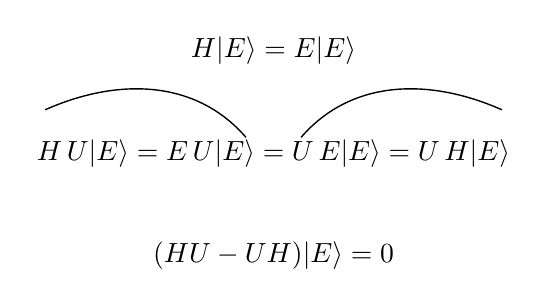
\begin{tikzpicture}
\node at (0,2.7) {$H|E\rangle = E|E\rangle$};
\node at (0,1.4) {$H\,U|E\rangle = E\,U|E\rangle = U\,E|E\rangle = U\,H|E\rangle$};
\node at (0,0.1) {$(HU-UH)|E\rangle = 0$};
\draw[line width=0.5pt] (-2.9,1.95) .. controls (-2.0,2.35) and (-1.0,2.35) .. (-0.35,1.6);
\draw[line width=0.5pt] (2.9,1.95) .. controls (2.0,2.35) and (1.0,2.35) .. (0.35,1.6);
\end{tikzpicture}
\caption{A clean companion reconstruction of the board derivation; the curved strokes only echo the lecture's guide marks.}
\end{figure}

If this annihilates every energy eigenstate, and if the energy eigenstates form a complete basis, then the operator itself must vanish:
\begin{equation}
[U,H]=0.
\end{equation}
That is the mathematical criterion for a symmetry transformation.

Now return to the infinitesimal form
\begin{equation}
U(\epsilon)=1+i\epsilon L_i+O(\epsilon^2).
\end{equation}
Since the identity commutes with everything, the same statement tells us that the generators commute with the Hamiltonian:
\begin{equation}
[L_i,H]=0.
\end{equation}
The lower board label in the surviving frame is a little soft, but the normalized form \([L_i,H]=0\) is the safest and most coherent way to write the lecture's conclusion.

\begin{figure}[t]
\centering

\includegraphics[width=0.45\textwidth]{lecture_04_figure_06.png}
\caption{Symmetry operators and generators commuting with the Hamiltonian. The upper relation is fully legible; the lower one is standardized cautiously as \([L_i,H]=0\).}
\end{figure}

This is more than a static condition. If an operator commutes with the Hamiltonian, then in the Heisenberg sense it is time-independent:
\begin{equation}
[O,H]=0
\qquad \Longrightarrow \qquad
\dot O = 0.
\end{equation}
Thus symmetry and conservation law stand very close to each other.

The lecture immediately cashes this out in the familiar example of atomic states. Fix the total angular momentum \(l\). The different magnetic quantum numbers \(m\) are rotated into one another, so they must all have the same energy:
\begin{equation}
E_{l,m}=E_l.
\end{equation}
That is precisely the content of rotational symmetry, provided there is no external magnetic or electric field to spoil it.

\subsection{Question \& Answer}

\paragraph{What counts as a true symmetry?}

This is where the lecture corrects a very common mistake. Suppose we rotate a spin in empty space. Its energy does not change. Good: rotation is a symmetry.

Now put that same spin in a magnetic field and rotate only the spin. Its energy changes. Does that mean rotation is not a symmetry? No. It means we did not perform the symmetry transformation. We rotated one part of the setup relative to another part that we held fixed. A genuine symmetry operation would rotate the spin and the magnetic field together.

The same point appears again for translation. An electron in the field of a proton does not keep the same energy if we translate only the electron. But that is not the symmetry operation either. Translating the whole electron-proton system is the symmetry. So when we say that symmetry does not change the energy, we mean a transformation of the whole physical configuration, not an isolated manipulation of one subsystem inside a fixed background.

\section{Why Supersymmetry Is Different}

Only after the entire review of ordinary symmetry does the lecture introduce the new idea. All symmetries discussed so far have one common feature: they preserve particle type. Rotating an electron gives an electron. A color transformation turns a quark into another quark. A scalar goes to a scalar; a spin-\(\tfrac12\) particle goes to another spin-\(\tfrac12\) particle. The symmetries may mix internal labels, spatial orientations, or magnetic quantum numbers, but they do not turn bosons into fermions.

Supersymmetry breaks exactly that pattern. It is a symmetry whose generators take bosons into fermions and fermions into bosons. The lecture presents this as a real escalation, not as one more example on the same list. Ordinary symmetry multiplets are already familiar: rotational symmetry forces the states with different \(m\)-values inside a fixed \(l\)-multiplet to have the same energy. Supersymmetry proposes a new kind of multiplet, one that crosses the boson-fermion divide.

The physical motivation is also kept in view. If a theory truly has supersymmetry, then bosons and fermions come in matched partners of equal mass. That is precisely the structure one would want if bosonic and fermionic contributions are to cancel the large renormalization effects discussed earlier in the course. So the lecture does not motivate supersymmetry by elegance alone. It motivates it by the possibility of a dynamical payoff.

\section{Supersymmetry Generators And Statistics}

The lecture now asks the central constructive question: what sort of operator could take a boson into a fermion and a fermion into a boson?

Let \(A\) and \(A^\dagger\) be bosonic annihilation and creation operators, and let \(C\) and \(C^\dagger\) be the corresponding fermionic operators. Then a simple prototype is
\begin{equation}
Q = C^\dagger A + A^\dagger C.
\end{equation}
The first term annihilates a boson and creates a fermion. The second annihilates a fermion and creates a boson. Schematically,
\begin{equation}
Q|B\rangle \sim |F\rangle,
\qquad
Q|F\rangle \sim |B\rangle.
\end{equation}

A student asks whether this means we are somehow creating a mysterious boson-fermion superposition as a single state. The lecture corrects that immediately. \(Q\) is an operator, not a state. Acting on a general superposition it may of course produce another superposition, but that is just the ordinary linearity of operators. The distinctive property is simpler: acting on a boson it gives a fermion, and acting on a fermion it gives a boson.

\subsection{Question \& Answer}

\paragraph{What happens when \(Q\) acts on the vacuum?}

This is the natural place to make a mistake, so the lecture stops and checks it explicitly.

Apply
\begin{equation}
Q = C^\dagger A + A^\dagger C
\end{equation}
to the vacuum \(|0\rangle\). The operator \(A\) tries to annihilate a boson, but no boson is present. The operator \(C\) tries to annihilate a fermion, but no fermion is present either. Therefore
\begin{equation}
Q|0\rangle = 0.
\end{equation}
This is not the vacuum again. It is the zero vector. The lecture is explicit about that distinction.

The next question is about spin. If a spin-zero boson is mapped to a fermion, which fermion appears? A spin-\(\tfrac12\) fermion has two components. So a single unindexed generator cannot be enough. The lecture's answer is that supersymmetry generators must carry a spinor index:
\begin{equation}
Q_\alpha.
\end{equation}
Schematically one should think of
\begin{equation}
Q_\alpha |B\rangle \sim |F_\alpha\rangle,
\qquad
Q_\alpha |F_\beta\rangle \sim \delta_{\alpha\beta}|B\rangle.
\end{equation}
The precise coefficients are not the point here. The point is that the generator itself carries half-integer spin because it changes spin by half a unit.

This already marks supersymmetry out as different from ordinary observables. Supersymmetry generators are fermionic operators: they contain an odd number of fermion operators. That is exactly why they can change bosons into fermions and fermions into bosons.

To see how radical this is, the lecture reviews the algebra of bosonic and fermionic creation and annihilation operators. For bosons we normalize the relations as
\begin{equation}
[A_i,A_j]=0,
\qquad
[A_i^\dagger,A_j^\dagger]=0,
\qquad
[A_i,A_j^\dagger]=\delta_{ij}.
\end{equation}
Hence bosonic creation operators commute:
\begin{equation}
A_i^\dagger A_j^\dagger = A_j^\dagger A_i^\dagger.
\end{equation}
So a two-boson state is symmetric under interchange of the labels \(i\) and \(j\).

For fermions we replace commutators by anticommutators:
\begin{equation}
\{C_i,C_j\}=0,
\qquad
\{C_i^\dagger,C_j^\dagger\}=0,
\qquad
\{C_i,C_j^\dagger\}=\delta_{ij}.
\end{equation}
In particular,
\begin{equation}
(C^\dagger)^2=0,
\end{equation}
which is the Pauli exclusion principle in operator form: two fermions cannot occupy the same state. And for distinct labels,
\begin{equation}
C_i^\dagger C_j^\dagger = -\,C_j^\dagger C_i^\dagger.
\end{equation}
So fermionic two-particle states are antisymmetric under exchange.

This is the point at which the lecture broadens again. Bosonic field amplitudes can become large and classical-looking. Fermionic objects cannot, because their squares vanish. That is what forces us toward a new kind of arithmetic.

\section{Grassmann Numbers}

The lecture introduces Grassmann numbers as the bookkeeping language appropriate to fermionic quantities and, in particular, to supersymmetry generators. Ordinary numbers commute:
\begin{equation}
\alpha_i\alpha_j=\alpha_j\alpha_i.
\end{equation}
Grassmann numbers anticommute:
\begin{equation}
\theta_i\theta_j=-\,\theta_j\theta_i.
\end{equation}
Setting \(i=j\) gives
\begin{equation}
\theta_i^2=0.
\end{equation}
And ordinary numbers commute with Grassmann numbers:
\begin{equation}
\alpha\theta=\theta\alpha.
\end{equation}

The lecture is careful not to overinterpret these objects. They are not directly measurable quantities. They are a new algebraic device. It is also careful about parity. A single \(\theta\) is odd. A product such as \(\theta_1\theta_2\) is even, in the graded sense that it commutes with other even quantities, but it need not be an ordinary scalar in the naive sense, because it may still be nilpotent.

With one Grassmann variable \(\theta\), the most general function is
\begin{equation}
f(\theta)=\alpha+\beta\theta.
\end{equation}
There is no quadratic term because \(\theta^2=0\). With two Grassmann variables,
\begin{equation}
f(\theta_1,\theta_2)=\alpha+\beta_1\theta_1+\beta_2\theta_2+\gamma\theta_1\theta_2.
\end{equation}
That is already the most general polynomial. The lecture lingers over how little room there is in this algebra.

Differentiation is then introduced with just one twist. For one variable we define
\begin{equation}
\partial_\theta(\alpha+\beta\theta)=\beta.
\end{equation}
For two variables we obtain
\begin{equation}
\partial_{\theta_1}f=\beta_1+\gamma\theta_2,
\qquad
\partial_{\theta_2}f=\beta_2-\gamma\theta_1.
\end{equation}
The minus sign in the second formula is the whole point. The derivative operator with respect to a Grassmann variable is itself Grassmann-odd, so when it passes through another Grassmann quantity it picks up a sign. The lecture emphasizes that this is precisely what is needed to preserve the usual product rule of calculus.

The one-variable exponential remains simple:
\begin{equation}
e^{a\theta}=1+a\theta.
\end{equation}
Therefore
\begin{equation}
e^{a\theta}e^{b\theta}=e^{(a+b)\theta}.
\end{equation}
Up to this point the algebra behaves exactly as the lecture hopes.

But then the lecture tries two Grassmann variables and the tone changes from exposition to investigation. One certainly computes
\begin{equation}
e^{\theta_1}e^{\theta_2}=(1+\theta_1)(1+\theta_2)=1+\theta_1+\theta_2+\theta_1\theta_2.
\end{equation}
The tempting next step is to compare this with \(e^{\theta_1+\theta_2}\). Here the lecture runs into a real puzzle. Because \((\theta_1+\theta_2)^2\) brings in \(\theta_1\theta_2+\theta_2\theta_1\), the naive exponential law becomes slippery. The discussion does not settle the matter. It is important not to flatten this into a polished theorem that the lecture itself never reached. The honest endpoint is that Grassmann arithmetic exists, is useful, and is essential, but the multi-variable exponential is left here as an unresolved question.

The lecture closes this part by noting that integration over Grassmann variables can also be defined, and that because the space of functions is so small the whole integration table will be correspondingly short. But that development is postponed. What matters for now is the existence of a consistent algebraic framework in which fermion operators and supersymmetry generators naturally live.

\section{Summary}

The lecture unfolds in a very deliberate order. We first rebuild the ordinary notion of symmetry: a unitary operator acting on states, with infinitesimal generators that close under commutation. We then learn to read the whole local structure of a continuous group from those commutators. Next comes the dynamical condition that turns transformation theory into symmetry theory:
\begin{equation}
[U,H]=0,
\qquad
[L_i,H]=0.
\end{equation}
Only after that groundwork is laid does supersymmetry appear, not as one more ordinary symmetry, but as a new sort of transformation that mixes bosons and fermions. That step forces us beyond ordinary commuting quantities and into Grassmann arithmetic. The lecture therefore ends, quite appropriately, not with a closed formal system, but with the sense that a new algebra has opened up and that supersymmetry lives at its center.